\subsection{System Modeling}
This section provides a visual and structured representation of the functional behavior of the aBridgeAI system. The system is modeled using Unified Modeling Language (UML) artifacts, primarily Use Case Diagrams, to describe how each actor interacts with the major functional modules of the platform.

The system is decomposed into eight functional modules: Authentication and Access Control, Organization and User Management, Course and Material Management, Learning Loop and Adaptive Quiz, Application Loop and Mock Interview, Analytics, Reporting and Notifications, Learning Programs and Path Governance, and Platform Configuration and Policy Documents.

% ==========================================
\subsubsection{Overall Use Case Diagram}

The Overall Use Case Diagram provides a macroscopic view of the aBridgeAI system boundary and the major interactions between the system and its authorised actors. The primary actors include Students, Teachers, Educational Managers, Faculty Deans, and IT Administrators. A Faculty Dean inherits every use case available to an Educational Manager within their faculty, so the diagram shows only the governance use cases that are distinctively theirs.



\begin{figure}[H]
    \centering
    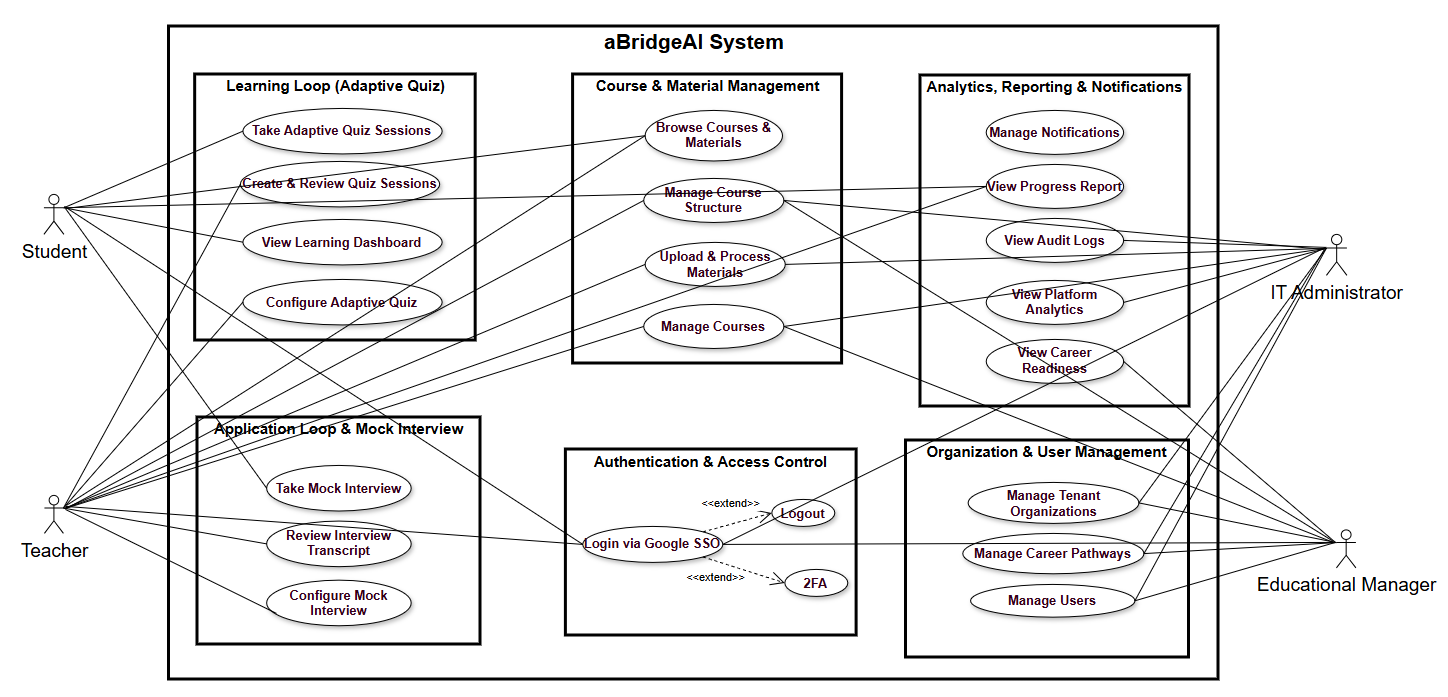
\includegraphics[width=0.95\textwidth]{graphics/usecase-diagrams/overall_usecase.png}
    \caption{Overall Use Case Diagram of the aBridgeAI System}
    \label{fig:overall_usecase}
\end{figure}

\noindent\textit{Note.} In this diagram, authentication is treated as a prerequisite for all protected use cases rather than as a repeated \textit{<<include>>} relationship.

% ==========================================
\subsubsection{Detailed Use Case Diagrams and Use Case Specifications}

The detailed use case diagrams decompose the overall system into module-level views. Each module-level diagram is followed by use case specifications that illustrate the most important workflows of that module. To keep the main report concise, only the most critical use cases are described in this section. The complete set of use case specifications is provided in Appendix~\ref{appendix:usecase-specifications}.


% ================1 Authentication and Access Control Module==========================
\paragraph{Authentication and Access Control Module}

This module covers Google SSO authentication, logout, authenticated session management, multi-factor authentication, role-based and permission-based access control, and security-related audit events.

The diagram highlights that all users must authenticate before accessing protected features. It also shows that sensitive account-security operations require recent second-factor verification, while access to backend routes and frontend UI actions is controlled by the authenticated user's active roles and effective permissions.

\begin{figure}[H]
    \centering
    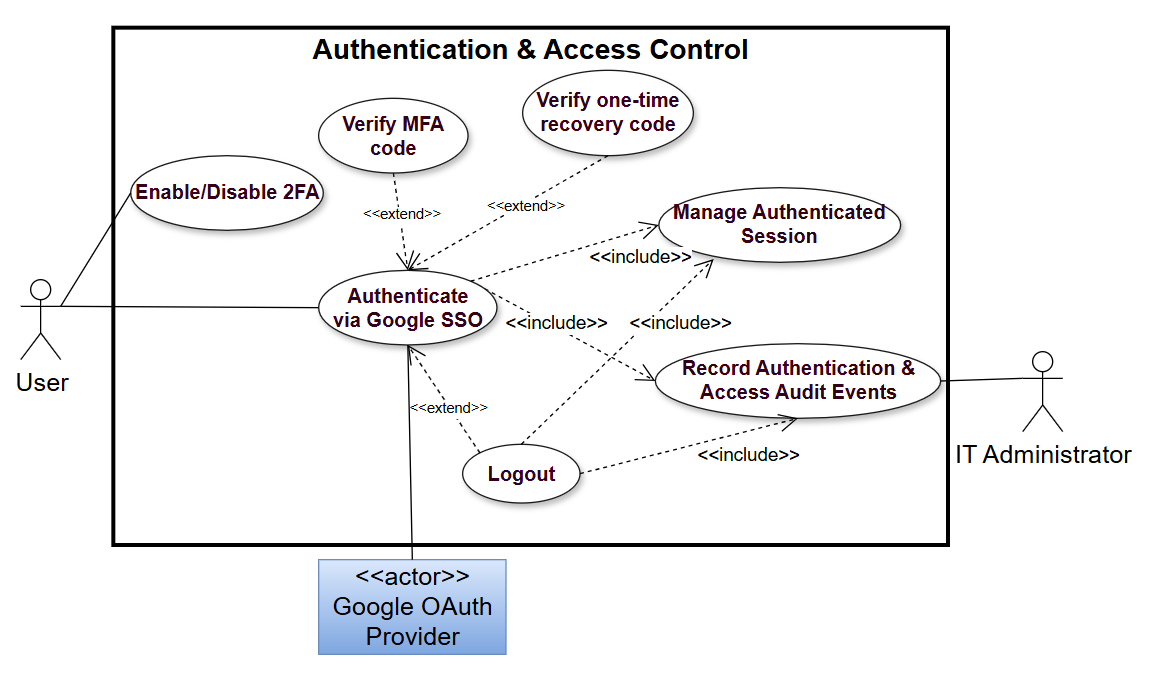
\includegraphics[width=0.7\textwidth]{graphics/usecase-diagrams/auth_access_usecase.png}
    \caption{Detailed Use Case Diagram: Authentication and Access Control Module}
    \label{fig:auth_access_usecase}
\end{figure}

The full set of use case specifications for this module is provided in Appendix~\ref{appendix:usecase-specifications}.



% 
% ===============2 Organization and User Management Module===========================
\paragraph{Organization and User Management Module}

This module supports multi-tenant organisation management, user onboarding, organisation memberships, user profiles, domain-based auto-provisioning, and tenant-scoped access control.

IT Administrators are responsible for provisioning and managing tenant organisations, organisation domains, and account status. Educational Managers manage learning operations such as bulk student enrolment, teacher-course assignment, and pathway administration within the organisation or faculty scope resolved from their permissions. The module ensures that Educational Manager actions and queries remain tenant-scoped.

\begin{figure}[H]
    \centering
    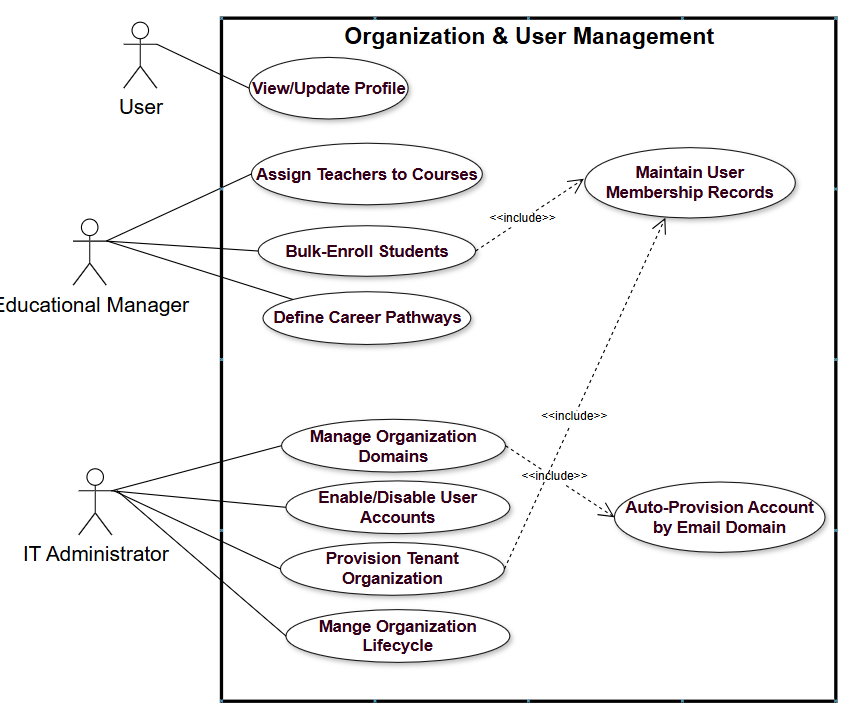
\includegraphics[width=0.7\textwidth]{graphics/usecase-diagrams/org_user_usecase.png}
    \caption{Detailed Use Case Diagram: Organization and User Management Module}
    \label{fig:org_user_usecase}
\end{figure}

\noindent The use case specifications for this module --- including tenant organisation management, which exercises the provisioning, lifecycle and domain-attachment flows in full --- are given in Appendix~\ref{appendix:usecase-specifications}.


% ==========================================
% ==========================================
\paragraph{Course and Material Management Module}

This module allows Teachers and Educational Managers to manage course lifecycles, organise modules and learning items, configure prerequisites and unlock rules, upload materials, manage material versions, and monitor ingestion progress.

The diagram also shows the student-facing side of the module, where enrolled Students can browse published courses, view course details, and access approved materials. Material visibility is controlled separately from course publication status, ensuring that students only access content that is both published and explicitly marked visible.

\begin{figure}[H]
    \centering
    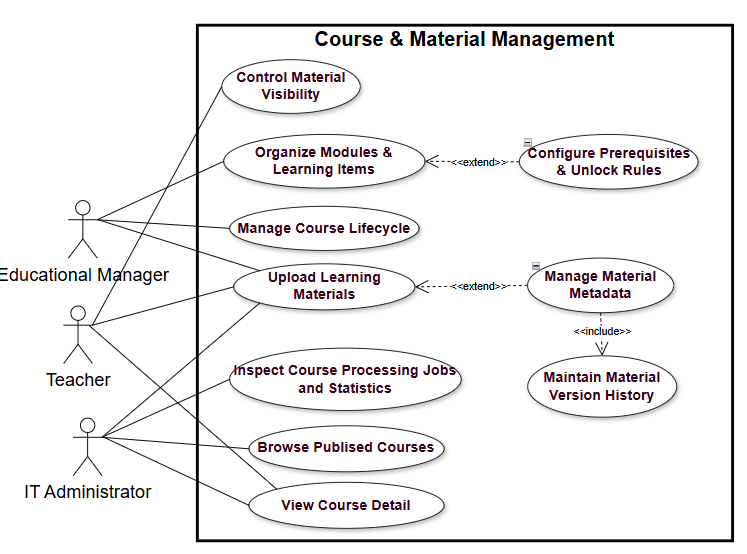
\includegraphics[width=0.7\textwidth]{graphics/usecase-diagrams/course_material_usecase.png}
    \caption{Detailed Use Case Diagram: Course and Material Management Module}
    \label{fig:course_material_usecase}
\end{figure}

\noindent The use case specifications for this module --- including the upload and ingestion workflow for learning materials --- are given in Appendix~\ref{appendix:usecase-specifications}.


% =====================4 Learning Loop and Adaptive Quiz Module =====================
\paragraph{Learning Loop and Adaptive Quiz Module}

This module represents the core learning mechanism of aBridgeAI, combining AI-assisted quiz question authoring, teacher review, adaptive quiz attempts, quality-score derivation, and hybrid SM-2 spaced-repetition scheduling.

Teachers create or review quiz questions, configure expected response time $T_{\text{exp}}$, spaced-repetition parameters, unlock thresholds, and prerequisites, and may require a camera for a given quiz. Students take quiz sessions, during which correctness, hint usage, and response time are recorded. These values are used to derive the per-card quality score $Q$ and update each student's spaced-repetition state. A live attempt admits only one client at a time, with the learner able to transfer it to another device by explicit confirmation; where a camera is required, the current implementation checks only that an active video track is present and keeps the stream local to the browser. The module also supports lesson access gating, due-card reminders, remediation links, and learning-loop dashboards.

\begin{figure}[H]
    \centering
    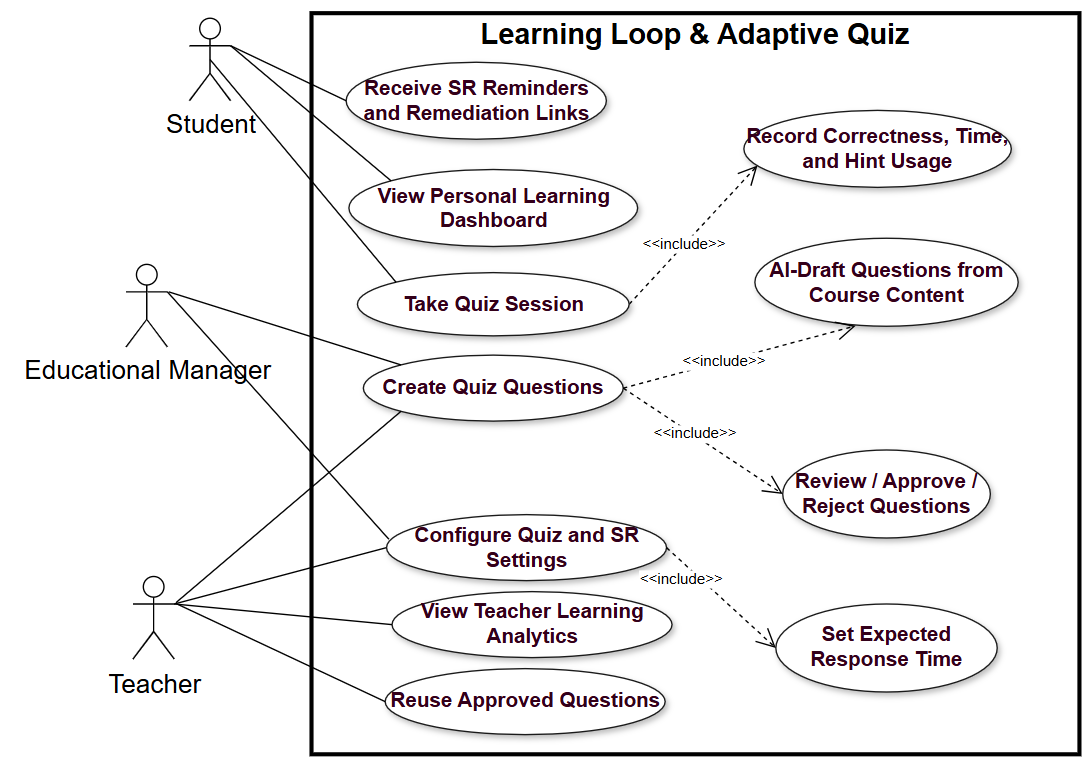
\includegraphics[width=0.70\textwidth]{graphics/usecase-diagrams/learning_loop_usecase.png}
    \caption{Detailed Use Case Diagram: Learning Loop and Adaptive Quiz Module}
    \label{fig:learning_loop_usecase}
\end{figure}

\noindent The use case specifications for this module --- including the adaptive quiz workflow, with $Q$ derivation and hybrid SM-2 scheduling --- are given in Appendix~\ref{appendix:usecase-specifications}.



% ===================5 Application Loop and Mock Interview Module=======================
\paragraph{Application Loop and Mock Interview Module}

This module focuses on transforming learned knowledge into applied interview performance. Teachers define desired outcomes that students must demonstrate, while the system can draft questions from ingested course content or accept manually authored questions. Each question may be linked to one desired outcome; unlinked questions and incomplete outcome coverage produce readiness warnings rather than universally preventing publication.

Students participate in mock interviews through a unified hybrid session supporting typed and spoken turns. The system persists the interview transcript and session metadata, then evaluates recorded answer evidence against teacher-defined desired outcomes asynchronously. After successful evaluation, students receive a binary pass-or-fail verdict together with a qualitative gap report and study plan; numeric rubric scores, per-outcome verdicts, and model reasoning remain hidden. Pending, recovery, and terminal evaluation-failure states do not invent a verdict. Teachers can review the transcript and outcome-level assessment for remediation purposes. The module also records browser activity signals to support post-session integrity review; these signals support human review but do not constitute conclusive evidence of misconduct or automatically terminate an interview.

Because the assessment is conducted through a conversational model, the module additionally guards the exchange in both directions: learner input is screened for prompt-injection attempts, and model output is screened for leakage of protected content before it reaches the learner. The guard defaults to shadow mode, which assesses and records security signals without changing learner-facing flow. Explicit enforcement configuration may refuse, redirect, or end the relevant turn rather than failing the whole session. Redacted security events are persisted, and authorised review is scope- and permission-controlled without exposing raw attack content. In the deployed configuration, a native LiveKit agent maintains conversational context while server-side selectors, state writers, and tool gates retain authority over progression. A routed legacy progression path remains available as a rollback configuration rather than the normal spoken-turn path.

\begin{figure}[H]
    \centering
    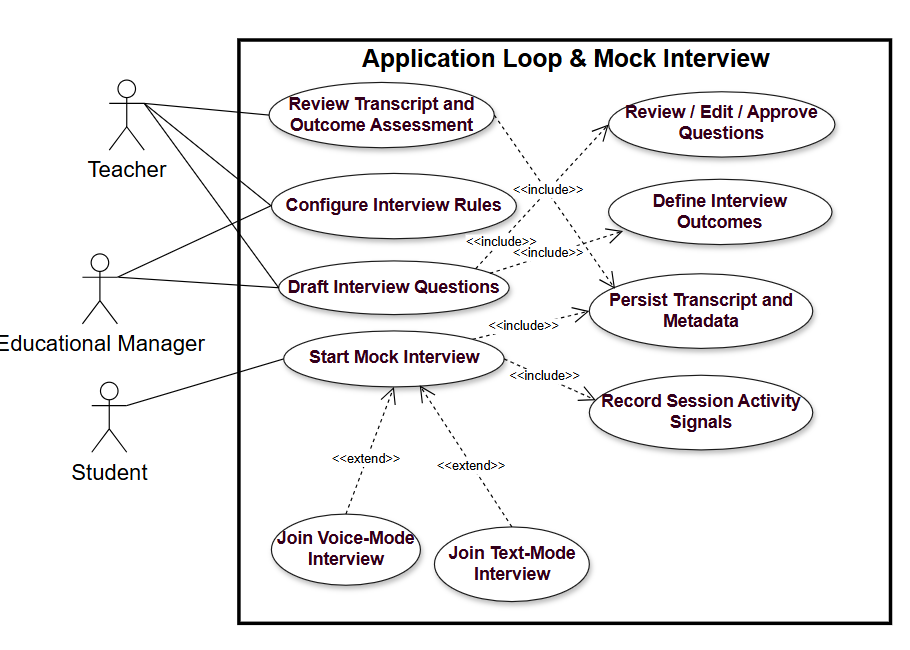
\includegraphics[width=0.70\textwidth]{graphics/usecase-diagrams/mock_interview_usecase.png}
    \caption{Detailed Use Case Diagram: Application Loop and Mock Interview Module}
    \label{fig:mock_interview_usecase}
\end{figure}

The full set of use case specifications for this module is provided in Appendix~\ref{appendix:usecase-specifications}.





% ====================6 Analytics, Reporting and Notifications Module======================
\paragraph{Analytics, Reporting and Notifications Module}
This module consolidates progress tracking, notification delivery, administrative analytics, audit-log querying, AI cost telemetry, processing-job inspection, and Career Readiness reporting.

Students can view completion progress and receive notifications, while Teachers can monitor roster progress and identify at-risk learners. Educational Managers can view organisation-scoped Career Readiness snapshots and drill down into individual learner progress. IT Administrators can inspect platform statistics, AI usage, processing jobs, and append-only audit records retained under the configured retention policy for security and compliance review.

\begin{figure}[H]
    \centering
    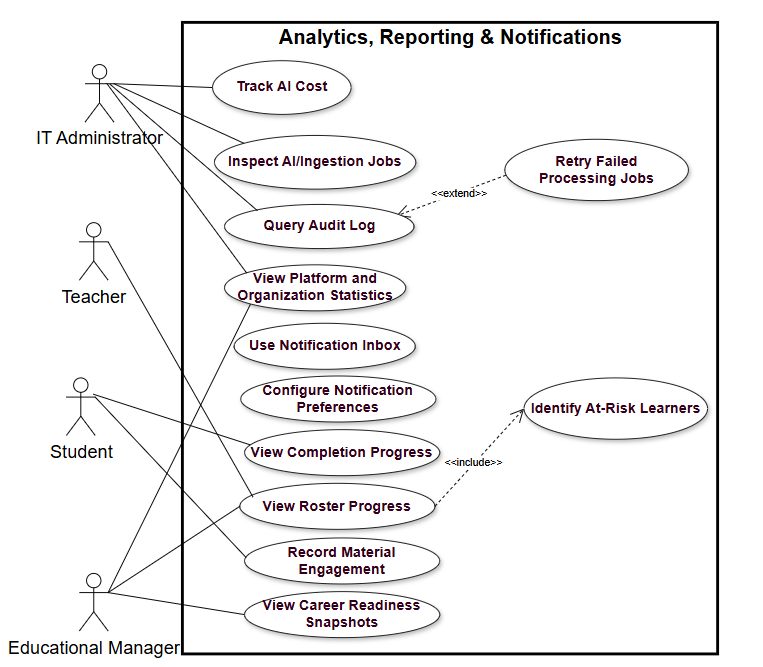
\includegraphics[width=0.70\textwidth]{graphics/usecase-diagrams/analytics_reporting_usecase.png}
    \caption{Detailed Use Case Diagram: Analytics, Reporting and Notifications Module}
    \label{fig:analytics_reporting_usecase}
\end{figure}
The full set of use case specifications for this module is provided in Appendix~\ref{appendix:usecase-specifications}.

% ====================7 Learning Programs and Path Governance Module======================
\paragraph{Learning Programs and Path Governance Module}

This module governs the enrolment structure that sits above individual courses. A \textit{learning programme} bundles one or more career pathways into a single enrolment offered by a faculty, and this module covers programme authoring, versioning, student enrolment, pathway selection, and the dean-adjudicated workflow by which a student changes or relinquishes a pathway.

Faculty Deans and Educational Managers author programmes within their own faculty and move them through draft, published, and archived states. Authoring is version-based: an edit opens a new draft rather than mutating a published version, so a student who enrolled under version~2 continues to see version~2 for the life of their enrolment. Authorised operators enrol students individually or by bulk import, subject to an organisation-configurable ceiling on concurrent programme enrolments.

On the student-facing side a programme version nominates one of its pathways as the default, and enrolment attempts to activate a system-originated attempt on it when the path is eligible and the concurrent-path constraints permit. Otherwise the enrolment remains awaiting selection. A student may then take on further pathways without approval, up to a limit the programme sets, which may exceed neither the pathways it bundles nor an organisation-configurable ceiling. Relinquishing a pathway is governed rather than free: a student may request either a change of pathway or, holding more than one, that a pathway be dropped, in each case with a mandatory written justification. Both kinds share a single open request per enrolment and a single finite switch allowance, which an approval spends and nothing restores. A request is adjudicated by a Faculty Dean who owns the programme and who may not be the subject of it. Approval closes the outgoing attempt with a progress snapshot, opening a replacement attempt for a change and none for a drop; no approval may leave a student with no pathway in progress, that being a withdrawal rather than a pathway decision. Course completions already earned are preserved as immutable awards, so work shared between pathways is never repeated, and the enrolment completes only once every pathway the student holds is itself complete.

\noindent A dedicated rendered use case diagram for this module is not yet included; the programme authoring, conditional default-path activation, pathway selection, and dean-adjudicated change-request workflows are specified textually in Appendix~\ref{appendix:usecase-specifications}.


% ====================8 Platform Configuration and Policy Documents Module======================
\paragraph{Platform Configuration and Policy Documents Module}

This module covers the operational surfaces through which the platform itself is tuned and through which its governing documents are published. It comprises two related concerns: a catalogue of runtime-tunable settings, and a versioned store of policy documents.

Every setting declares its key, grouping, data type, default value, and description. The effective value of a setting is resolved by a fixed precedence of organisation override, deployment-wide stored value, environment configuration, and code default, so that an IT Administrator tunes the deployment while an Educational Manager tunes only their own organisation. Because a mis-set value can affect every tenant, a change may first be previewed as a validated dry run that reports what it would alter; every applied change carries a mandatory written reason and is recorded so that it can later be cleared or rolled back to the value it replaced. Should a stored setting become unreachable, unreadable, or invalid, the system falls through to the next precedence layer rather than failing.

Policy documents — each classified as legal or academic — hold their content in independently numbered versions, so that the text in force on a given date remains recoverable. The index of published policies and the current text of any published policy are served without requiring authentication, since a prospective user must be able to read the terms before holding an account.

\noindent A dedicated rendered use case diagram for this module is not yet included; runtime-setting precedence, preview, rollback, and policy-document workflows are specified textually in Appendix~\ref{appendix:usecase-specifications}.






% ======================Activity Diagrams===========================
\subsubsection{Activity Diagrams}

Activity diagrams model the dynamic behavior of the system by illustrating the flow of activities, decision points, and asynchronous AI-driven processes.
The system activity diagrams focus on four major workflows: Authentication, Smart Content Ingestion, Human-in-the-Loop Quiz Generation, and Context-Aware Mock Interviews.

The following activity diagram illustrates the Human-in-the-Loop quiz generation workflow. The full set of activity diagrams is provided in Appendix~\ref{appendix:activity-diagrams}.

\begin{figure}[H]
    \centering
    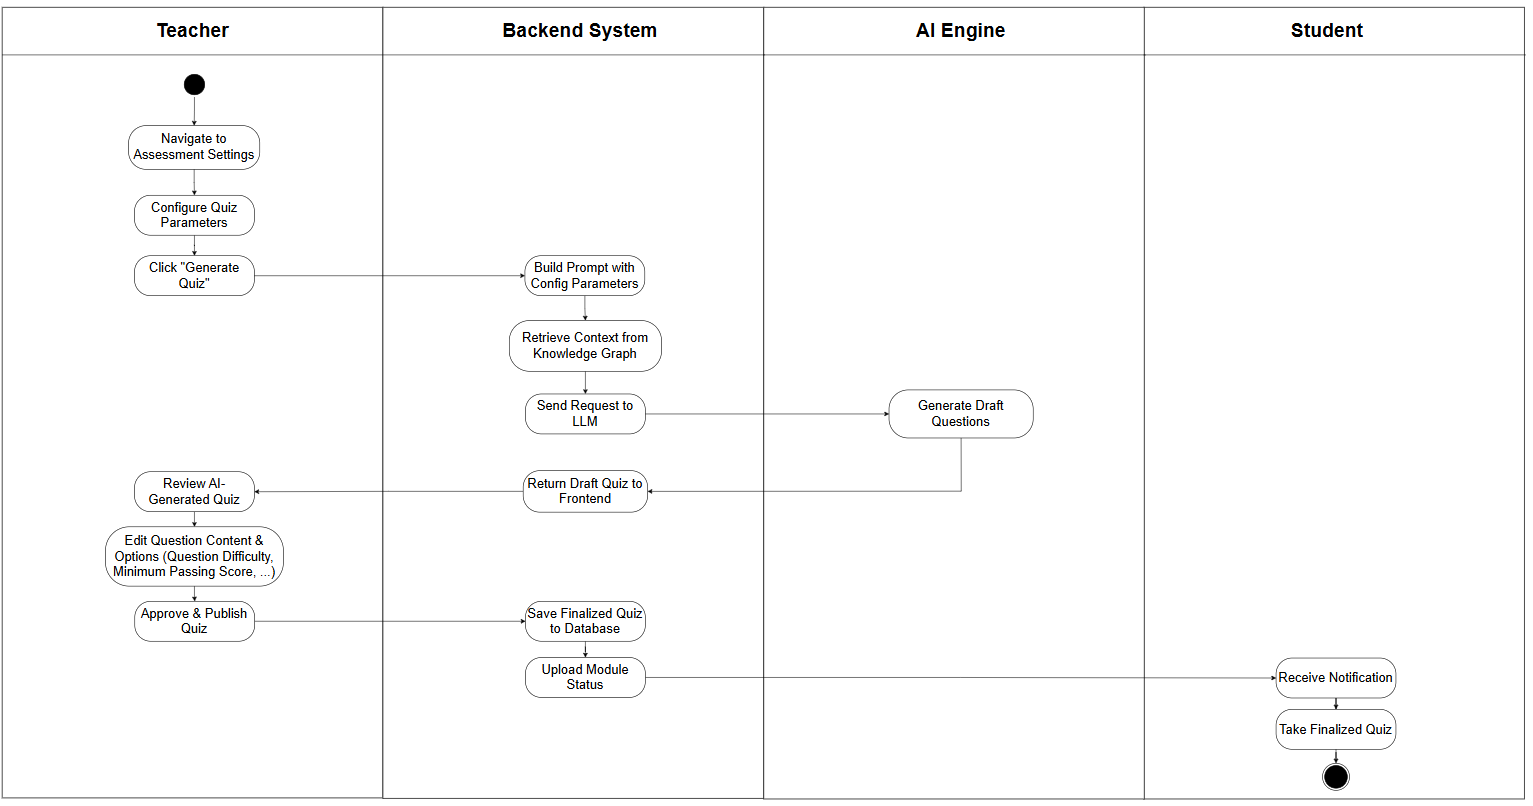
\includegraphics[width=1\textwidth]{graphics/act-diagrams/act_quiz_gen.png}
    \caption{Activity Diagram: HITL Quiz Generation and Execution}
    \label{fig:act_quiz_gen_rep}
\end{figure}

The following activity diagram details the material ingestion workflow in aBridgeAI. It shows how teachers upload learning materials directly to object storage, how the backend verifies the upload and queues processing, and how the ingestion worker extracts, chunks, embeds, and stores content for retrieval.

\begin{figure}[H]
    \centering
    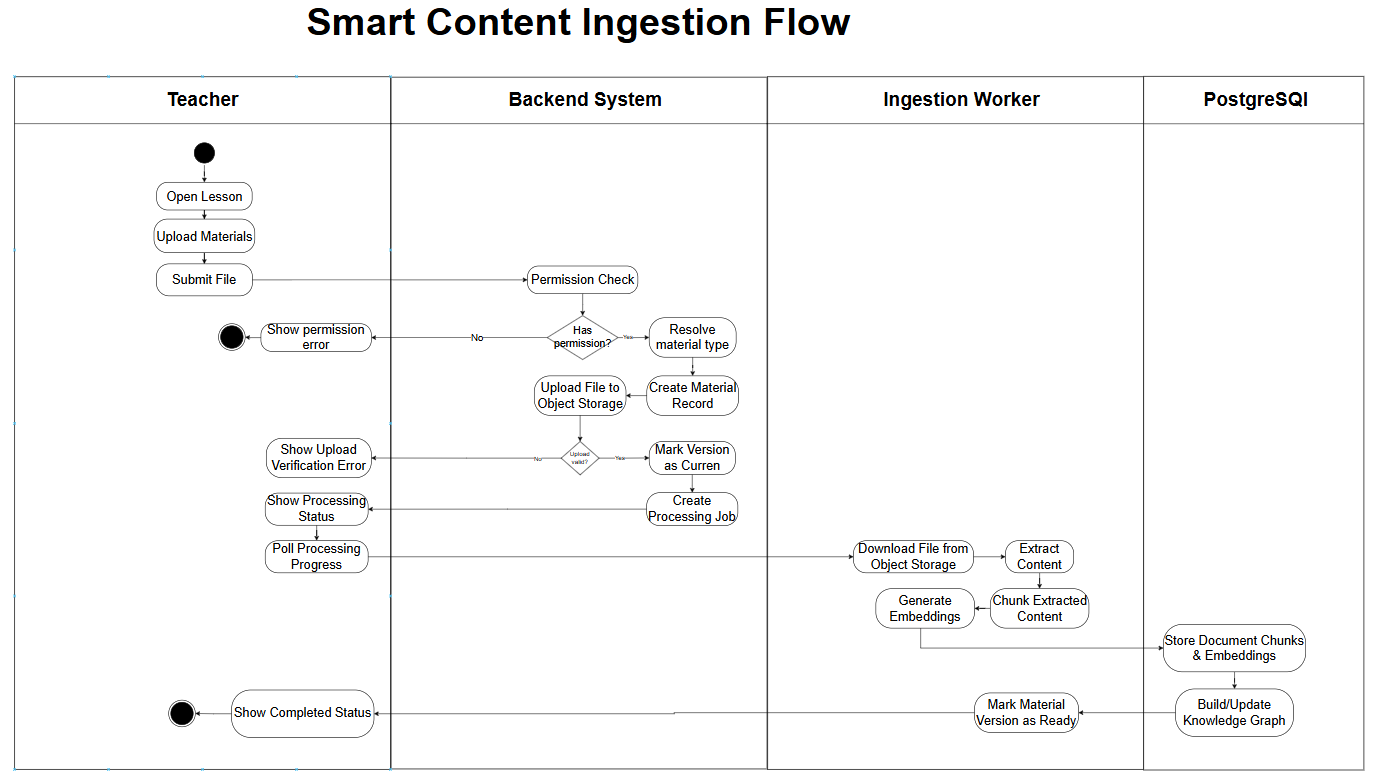
\includegraphics[width=0.95\textwidth]{graphics/act-diagrams/act_ingestion.png}
    \caption{Activity Diagram: Smart Content Ingestion and AI Parsing}
    \label{fig:act_ingestion_rep}
\end{figure}
Detailed activity diagrams are provided in Appendix~\ref{appendix:activity-diagrams}.
